
%%%%%%%%%%using figures to present incast: tput, fariness, droprate, TCP RTT

\begin{figure*}[!t]
        \centering
        \begin{subfigure}[b]{0.33\textwidth}
                \centering
                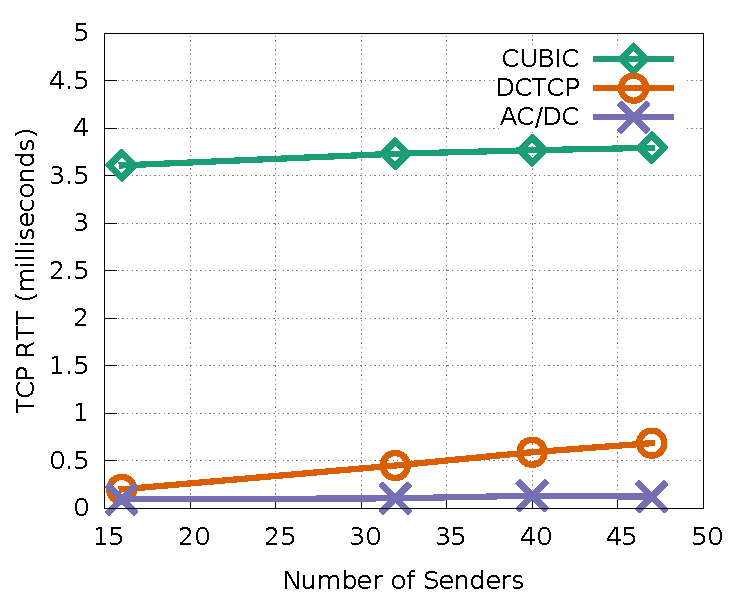
\includegraphics[width=\textwidth]{figures/incast/plots9k/incast_sockperf50th_vary_sender.pdf}
                \caption{50$^{th}$ percentile RTT ($\mu$s).}
                \label{incast_9k_50th_sockperf}
        \end{subfigure}
        \begin{subfigure}[b]{0.33\textwidth}
                \centering
                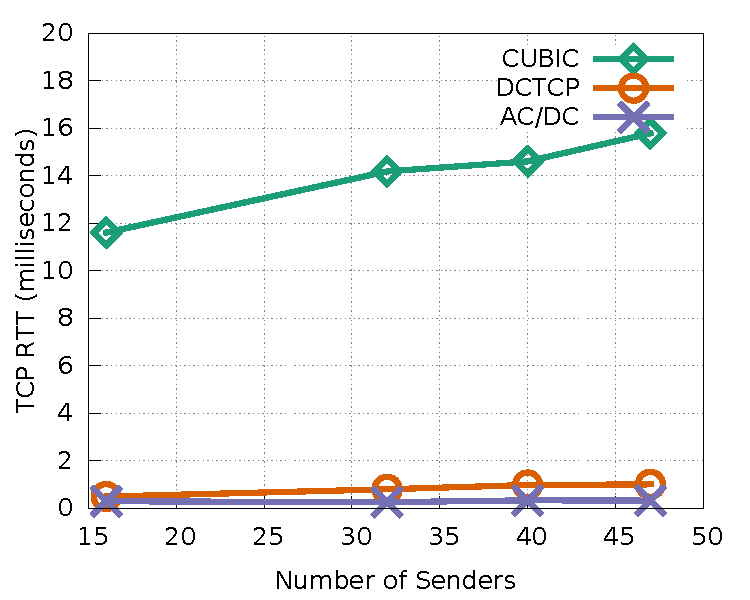
\includegraphics[width=\textwidth]{figures/incast/plots9k/incast_sockperf999th_vary_sender.pdf}
                \caption{99.9$^{th}$ percentile RTT ($\mu$s).}
                \label{incast_9k_999th_sockperf}
        \end{subfigure}
        \begin{subfigure}[b]{0.33\textwidth}
                \centering
                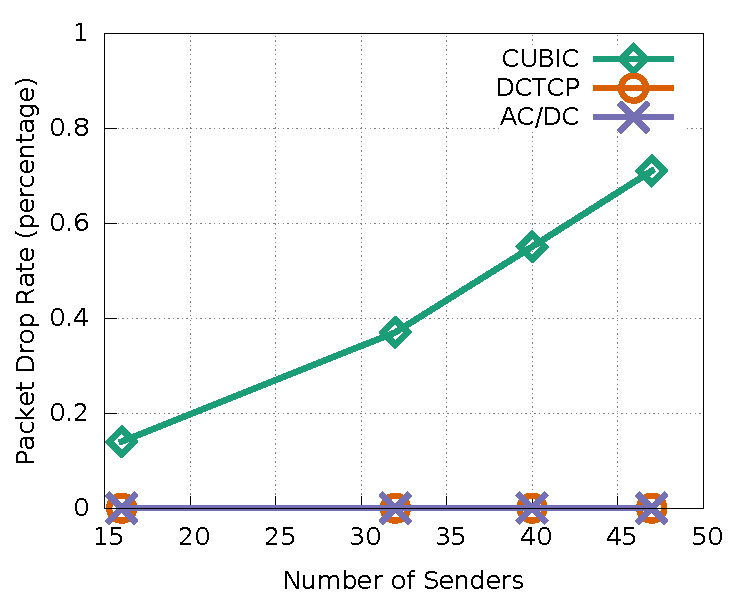
\includegraphics[width=\textwidth]{figures/incast/plots9k/incast_droprate_vary_sender.pdf}
                \caption{Packet drop rate.}
                \label{incast_9k_droprate}
        \end{subfigure}
	\caption{Many to one incast: RTT and packet drop rate.}
	\label{incast_9k_sockperf_droprate}
\end{figure*}

\begin{figure}[!t]
        \centering
        \begin{subfigure}[b]{0.225\textwidth}
                \centering
                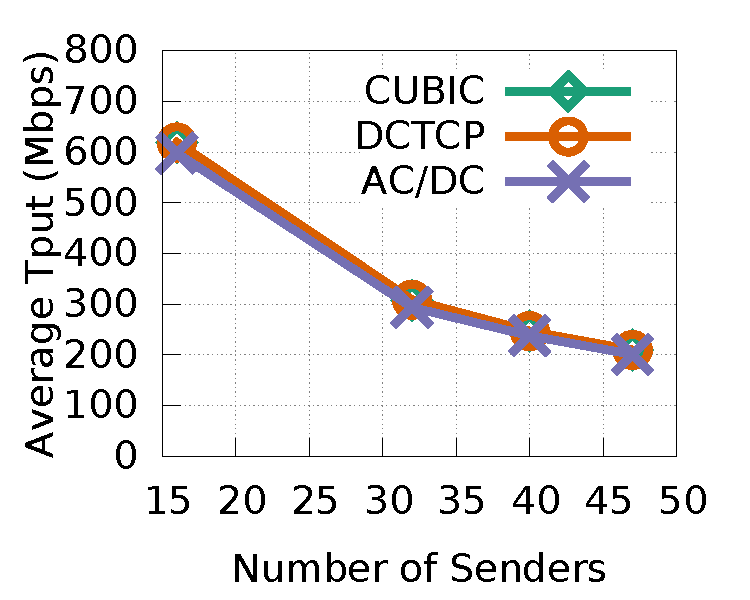
\includegraphics[width=\textwidth]{figures/incast/plots9k/incast_tput_vary_sender.pdf}
                \caption{Average throughput.}
                \label{incast_9k_tput}
        \end{subfigure}
        \begin{subfigure}[b]{0.225\textwidth}
                \centering
                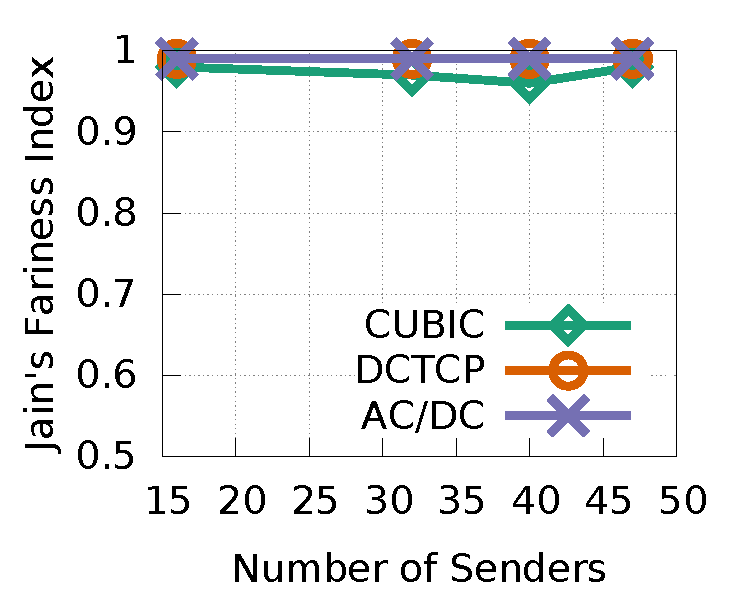
\includegraphics[width=\textwidth]{figures/incast/plots9k/incast_fairness_vary_sender.pdf}
                \caption{Fairness.}
                \label{incast_9k_fariness}
        \end{subfigure}
        \caption{Many to one incast: throughput and fairness.}
        \label{incast_9k_tput_fairness}
\end{figure}


%%%%47 to 1 incast, sockperf CDF %%%
%\begin{figure}[t]
%        \centering
%  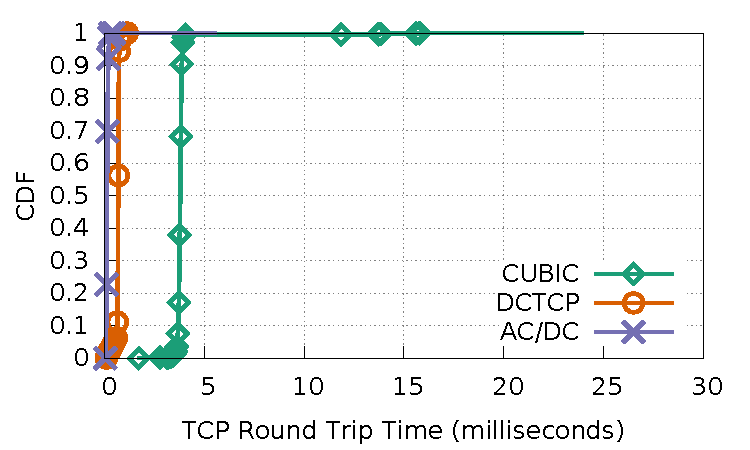
\includegraphics[width=0.45\textwidth]{figures/incast/47to1/incast_47to1_test_sockperf.pdf}
%        \caption{TCP RTT in 47 to 1 incast test.}
%        \label{sockperf_incast_47to1}
%\end{figure}

\begin{figure}[t]
        \centering
  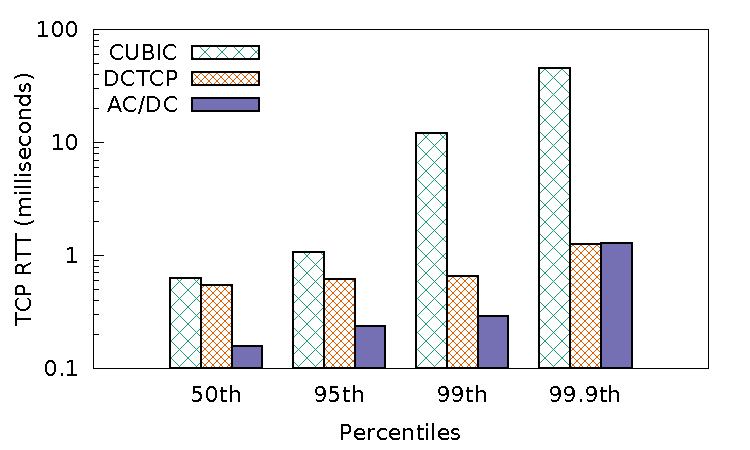
\includegraphics[width=0.45\textwidth]{figures/incast/pressure/incast_pressure_compare_sockperf.pdf}
        \caption{RTTs when almost all ports are congested.}
        \label{sockperf_pressure_incast}
\end{figure}


\tightparagraph{Incast}
In this section, we evaluate incast scenarios.
To scale the experiment, 17 physical servers are equipped with four NICs each
and one flow is allocated per NIC.
In this way, incast can support up to 47-to-1 fan-in (our switch only has 48 ports).
We measure the extent of incast by increasing the number of concurrent senders to 16, 32, 40 and 47.
Figure~\ref{incast_9k_tput_fairness} shows throughput and fairness results.
Both DCTCP and \acdc{} get comparable throughput as CUBIC and both offer a fairness index greater than 0.99.
Figure~\ref{incast_9k_sockperf_droprate} shows the TCP RTT and packet drop rate results.
When there are 47 concurrent senders, DCTCP can reduce median TCP RTT by 82\% and \acdc{} can reduce by 97\%;
DCTCP can reduce 99.9$^{th}$ percentile TCP RTT by 94\% and \acdc{} can reduce by 98\%.
Both DCTCP and \acdc{} have 0\% packet drop rate. It is curious that~\acdc{}’s
performance is better than DCTCP when the number of senders increases (Figure~\ref{incast_9k_50th_sockperf}).
The Linux DCTCP code puts a lower bound of 2 packets on \cwnd{}.
In incast, we have up to 47 concurrent competing flows and
the network's MTU size is 9kB. In this case, the lower bound is too high,
so DCTCP's RTT increases gradually with the number of senders.
This issue was also found in~\cite{judd2015nsdi}.~\acdc{} controls \rwnd{} (which is in bytes)
instead of \cwnd{} (which is in packets) and \rwnd{}'s lowest value can be much smaller than 2*MSS.
We verified modifying~\acdc{}'s lower bound caused identical behavior.


The second test checks whether \acdc{} can interact well with the switch's dynamic 
buffer allocation scheme. To this end, we aim to congest every switch port.
The 48 NICs are split into 2 groups: group $A$ and $B$. 
Group $A$ has 46 NICs and $B$ has 2 (denoted $B_1$ and $B_2$). 
Each of the 46 NICs in $A$ sends and receives 4 concurrent flows within $A$ 
(\ie{}, NIC $i$ sends to [$i+1$, $i+4$] mod 46). 
Meanwhile, all of the NICs in $A$ send to $B_1$, creating a 46-to-1 incast. 
This workload congests 47 out of 48 switch ports. 
We measure the TCP RTT between $B_2$ and $B_1$ (i.e., TCP RTT of the traffic traversing the most congested port) and 
the results are shown in Figure~\ref{sockperf_pressure_incast}. 
The average throughputs for CUBIC, DCTCP, and~\acdc{} are 214, 214 and 201 Mbps respectively, 
all with a fairness index greater than 0.98. 
CUBIC has an average drop rate of 0.34\% but the most congested port has a drop rate as high as 4\%. 
The packet drop rate for both DCTCP and~\acdc{} is 0\%.



%\iffalse
%%%% incast, 16 to 1 %%%
%% see , /power/home/keq/workloads/program/acdctcp/incast-container16-10Minutes
%\begin{table*}[!htb]
%\begin{center}
%\begin{tabular}{ |c|c|c|c|c|c| }
% \hline
%  & Avg Tput (Mbps) & Fairness Index & 50$^{th}$ percentile TCP RTT ($\mu$s) & 99.9$^{th}$ percentile TCP RTT ($\mu$s) & Drop Rate \\
% \hline
%
% Default & 619 & 0.98 & 3607 & 11599 & 0.14\% \\
% DCTCP  & 619 & 0.99 & 197 & 486 & 0 \\
% Ours & 598 & 0.99 &  93 & 289 & 0 \\
% \hline
%\end{tabular}
%\caption{16 to 1 incast test. MTU = 9000 B. Marking min = 10.}
%\label{incast_16to1_tbl_9000}
%\end{center}
%\end{table*}
%
%%see, /power/home/keq/workloads/program/acdctcp/incast-container32-10Minutes
%\begin{table*}[!htb]
%\begin{center}
%\begin{tabular}{ |c|c|c|c|c|c| }
% \hline
%  & Avg Tput (Mbps) & Fairness Index & 50$^{th}$ percentile TCP RTT ($\mu$s) & 99.9$^{th}$ percentile TCP RTT ($\mu$s) & Drop Rate \\
% \hline
%
% Default & 318 & 0.97 & 3729 & 14448 & 0.37\% \\
% DCTCP  & 319 & 0.99 & 448 & 792 & 0 \\
% Ours & 303 & 0.99 &  103 & 249 & 0 \\
% \hline
%\end{tabular}
%\caption{32 to 1 incast test. MTU = 9000 B. Marking min = 10.}
%\label{incast_32to1_tbl_9000_markingMin10}
%\end{center}
%\end{table*}
%
%%see, /power/home/keq/workloads/program/acdctcp/incast-container41
%\begin{table*}[!htb]
%\begin{center}
%\begin{tabular}{ |c|c|c|c|c|c| }
% \hline
%  & Avg Tput (Mbps) & Fairness Index & 50$^{th}$ percentile TCP RTT ($\mu$s) & 99.9$^{th}$ percentile TCP RTT ($\mu$s) & Drop Rate \\
% \hline
%
% Default & 245 & 0.96 & 3767 & 14596 & 0.55\% \\
% DCTCP  & 247 & 0.99 & 589 & 973 & 0 \\
% Ours & 238 & 0.99 &  130 & 327 & 0 \\
% \hline
%\end{tabular}
%\caption{40 to 1 incast test. MTU = 9000 B. Marking min = 10.}
%\label{incast_40to1_tbl_9000_markingMin10}
%\end{center}
%\end{table*}
%
%
%%see, /power/home/keq/workloads/program/acdctcp/incast-container48
%\begin{table*}[!htb]
%\begin{center}
%\begin{tabular}{ |c|c|c|c|c|c| }
% \hline
%  & Avg Tput (Mbps) & Fairness Index & 50$^{th}$ percentile TCP RTT ($\mu$s) & 99.9$^{th}$ percentile TCP RTT ($\mu$s) & Drop Rate \\
% \hline
%
% Default & 210 & 0.98 & 3792 & 15776 & 0.71\% \\
% DCTCP  & 210 & 0.99 & 684 & 1000 & 0 \\
% Ours & 201 & 0.99 &  121 & 314 & 0 \\
% \hline
%\end{tabular}
%\caption{47 to 1 incast test. MTU = 9000 B. Marking min = 10.}
%\label{incast_47to1_tbl_9000_markingMin10}
%\end{center}
%\end{table*}
%
%\fi
%
